\documentclass{article}
\usepackage[T1]{fontenc}
\usepackage{lmodern}
\usepackage{graphicx}
\usepackage{amsmath,amssymb}
\usepackage[a4paper,margin=2cm]{geometry}
\usepackage[absolute,overlay]{textpos}
\setlength{\TPHorizModule}{1mm}
\setlength{\TPVertModule}{1mm}
\usepackage[indonesian]{babel}
\usepackage{hyperref}
\setlength{\emergencystretch}{2em}
% unit: Halaman 30

\begin{document}

% === Halaman 30 (llm) ===

\vspace{95.04mm}

\section*{Sejarah Vigenere Cipher}

\begin{itemize}
    \item Penemu \textit{cipher} ini sebenarnya adalah Giovan Batista Belaso, karena ia menggambarkan pertama kali pada tahun 1553 seperti ditulis di dalam bukunya \textit{La Cifra del Sig. Giovan Batista Belaso}.
    \item Namun, \textit{cipher} ini disempurnakan dan dipublikasikan oleh diplomat (sekaligus seorang kriptologis) Perancis, Blaise de Vig\grave{e}nere pada abad 16 (tahun 1586).
    \item Pada abat ke-19, banyak orang yang mengira Vigen\grave{e}re adalah penemu \textit{cipher} ini, sehingga dikenal luas sebagai \textit{Vigen\grave{e}re Cipher}.
\end{itemize}

% deskripsi: Potret Blaise de Vigenère
% bbox normalisasi: [0.8370, 0.0050, 0.9720, 0.3250]
\begin{textblock*}{28.35mm}(175.77mm,1.49mm)
\noindent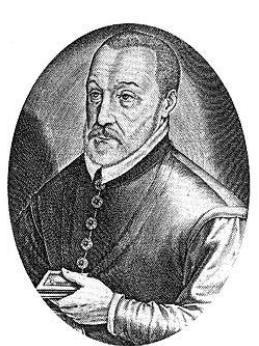
\includegraphics[width=28.35mm,height=95.04mm]{../../images/llm/page_030_img_01.png}%
\end{textblock*}

\end{document}
